\documentclass[12pt,a4paper]{article}
\usepackage[utf8]{inputenc}
\usepackage[T1]{fontenc}
\usepackage[francais]{babel}
\usepackage{amsmath}
\usepackage{amsfonts}
\usepackage{amssymb}
\usepackage{xcolor}
\usepackage{graphicx}
\usepackage[top=2.00cm]{geometry}
\usepackage{titlesec}
\usepackage{fancyhdr}
\usepackage{multicol}
\usepackage{titling}
\usepackage{mathtools}
\usepackage{appendix}
\renewcommand{\appendixpagename}{Annexes}
\renewcommand{\appendixtocname}{Annexes}
%\usepackage[hidelinks]{hyperref}
\usepackage[colorlinks = true,
linkcolor = blue,
urlcolor  = blue,
citecolor = blue,
anchorcolor = blue]{hyperref}
\graphicspath{{C:/Users/Sylvain/AppData/Roaming/texstudio/templates/user/}{./res/}}

%%modif des titres de section diminuer la taille
\renewcommand{\thesection}{\Roman{section}}
\titleformat{\section}
{\normalfont\bfseries\Large\scshape}{\thesection}{1em}{}
\titleformat{\subsection}
{\normalfont\bfseries\large}{\thesubsection}{1em}{}

\addto{\captionsfrench}{\renewcommand{\abstractname}{}}

%CONFIG
\author{Sylvain Finot}
\title{Initiation à la recherche :\\[1ex] \scshape Le Rattleback}
%\title{\scshape Étude du rattleback}
\date{\today}
\fancypagestyle{firststyle}{
	\fancyhf{}
	\setlength{\footskip}{2cm}
	\renewcommand{\headrulewidth}{0pt}
	\cfoot{\textcolor{lightgray}{\theauthor \ | Initiation à la recherche | Mars 2017}}
	\rfoot{\thepage}
}
\pagestyle{firststyle}

\makeatletter
\def\@maketitle{
	\begin{center}
		
		% NoLogo
		 \vspace*{+2cm}
		
		% Corner Logo
		% \begin{flushright}
		%  
\includegraphics[width=40mm]{logo_corner}\\[4ex]
		% \end{flushright}
		
		% Top Logo
		%
\includegraphics[scale=0.3]{logo_top}
		
		
		{\LARGE \@title }\\[4ex]
		{\large \@author}\\[4ex]
		{\large \@date}\\[8ex]
		\rule{\linewidth}{0.4pt}
	\end{center}
}


%matrices configurables \begin{pmatrix}[2pt]
\renewcommand*\env@matrix[1][\arraystretch]{%
	\edef\arraystretch{#1}%
	\hskip -\arraycolsep
	\let\@ifnextchar\new@ifnextchar
	\array{*\c@MaxMatrixCols c}}

%parenthèses eqref hyperref
\renewcommand*{\eqref}[1]{%
	\hyperref[{#1}]{\textup{\tagform@{\ref*{#1}}}}%
}
\makeatother


\begin{document}
	\maketitle
	\thispagestyle{firststyle}
	\begin{abstract}
		%todo mettre référence de American Journal of Physic
		Dans ce document, nous allons tenter d'expliquer au mieux l'étude du rattleback menée par William Case et Sahar Jalal.\\
		Leur article, \textit{"The rattleback revisited"}, paru dans The American Journal of Physics en 2014 traite du mouvement surprenant du rattleback. Bien que de nombreuses études aient été réalisées sur le rattleback, les auteurs mentionnent le fait que leur approche est beaucoup plus directe que celles déjà existantes au moment de la publication.\\
		
		Je vais donc essayer de traiter au mieux les points évoqués dans l'article et de synthétiser ce que j'ai compris avec mon niveau actuel de physique (3ème année de licence)
		%comprendre la démarche
		%voir les hypotheses
		%probleme LaTeX, beaucoup de temps si on veux etre precis
		%Rq: avec des bases de physique, on peut comprendre ce qui est fait sans forcement être capable de refaire tout les calculs.
	\end{abstract}
	\section{Introduction}
	Un rattleback, aussi appelé anagyre ou "Celtic stone", est un objet généralement en forme de canoë, qui a la particularité d'avoir un sens de rotation stable et un sens instable autour de l'axe vertical.
	\begin{figure*}[h]
		\centering
		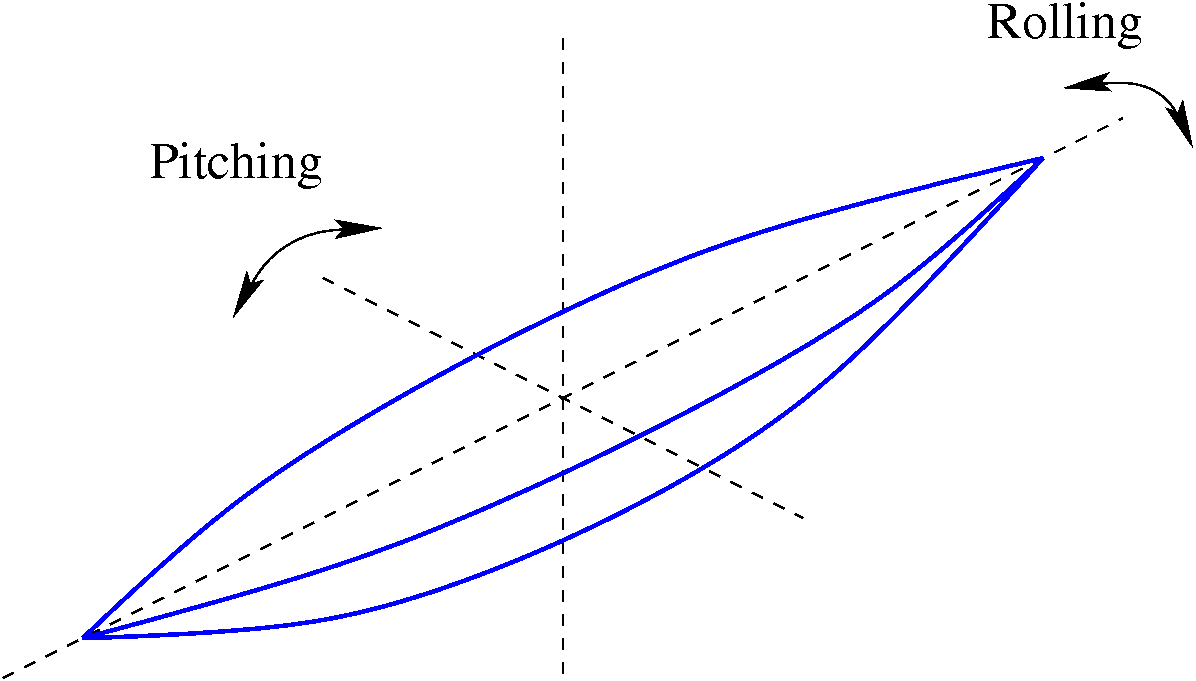
\includegraphics[scale=0.2]{Rolling-pitching}
		\caption[]{Représentation simpliste d'un rattleback}
		\label{fig:rolling-pitching}
	\end{figure*}
	
	Autrement dit, si on le met en rotation dans le "bon" sens, le mouvement continue jusqu'à immobilisation due aux forces de frottement. En revanche, si on le met en rotation dans le "mauvais" sens, très vite, l'objet oscille violemment ("rattle"), s'arrête, puis repart en sens inverse (i.e, le "bon" sens). Autre particularité, si on fait osciller le rattleback selon son petit axe (l'axe "pitching" \autoref{fig:rolling-pitching}), il entre en rotation dans le bon sens de rotation.
	
	Cet objet, par son mouvement paradoxal, est parfois retrouvé comme accessoire de magicien.
	Il a également fasciné grand nombre de physiciens et de mathématiciens. Les premières publications à ce sujet datent de 1896 par Gilbert Walker. La plupart des publications actuelles (XXI$^{e}$ siècle) se basent sur les travaux d'Hermann Bondi, "The Rigid Body Dynamics of Unidirectional Spin" de 1986.
	\subsection{Un problème de symétrie.}
	Bien que le mouvement du rattleback soit surprenant et fascinant, il n'y a rien de magique dans cet objet. Ses propriétés sont dues à un problème de symétrie. En effet, le rattleback est un objet asymétrique.
	
	Il existe deux manières de concevoir un rattleback : on peut décider de prendre une répartition de masse homogène, et dans ce cas, on brise la symétrie en modifiant le volume. On peut aussi choisir de conserver les symétries du volume et de "cacher" l'asymétrie en appliquant une répartition inhomogène de la masse avec par exemple des cavités. L'étude faite ici concerne le cas de répartition de masse homogène.
	
	\subsection{Démarche de l'étude}
	Afin de ne pas perdre le lecteur, je trouve important d'annoncer le plan de l'étude réalisée dans l'article.
	
	Le problème étant complexe, il est judicieux de découper l'analyse.
	La première partie consiste à étudier comment, à partir de rotation autour de l'axe vertical, le rattleback se met à osciller.
	Ensuite, les auteurs s'intéressent au cas contraire, c'est-à-dire, comment à partir d'oscillations le rattleback passe-t-il en rotation.
	
	C'est en réunissant les résultats des deux parties que l'on obtient une réponse relativement complète au problème.
	
	Avant de rentrer dans le vif du sujet, je précise que j'ai essayé de démontrer la plupart des résultats obtenus par les auteurs. Les étapes de calculs (situés dans la \autoref{sec:calculs}) seront indiquées en référence.
	% il faut faire un certain nombre d'hypothèses pour pouvoir espérer le résoudre.
	% %todo : HYPOTHESES
	% On considère que le point de contact entre le rattleback et le support est au repos.
	% %Conservation de l'E (28 29)
	% 
	% Pour simplifier le traitement du problème, on peut le découper en deux parties.\\
	%  %D'une certaine manière, on peut voir cela comme une conversion d'énergie.\\
	% La deuxième partie, on s'intéresse au cas contraire, comment à partir d'oscillations le rattleback passe-t-il en rotation.
	\section{Oscillations induites}
	Dans cette première partie de l'étude, sans doute la plus complexe, on considère que le rattleback est initialement en rotation selon l'axe vertical sans aucune oscillation. On cherche alors à expliquer pourquoi et comment ce mouvement se transforme en oscillation.
	%L'idée est de mettre en équation le changement 
	En ce qui concerne l'aspect calculs, il faudra tenir compte du fait que le référentiel du centre de masse est en rotation par rapport au référentiel du laboratoire.\\
	Le repère utilisé a pour origine le centre de masse et comme axes, les axes de symétrie (en terme de distribution de masse).\\
	\begin{figure}[h]
		\centering
		\caption{Le rattleback vu de dessus. La répartition de masse ne respecte pas la symétrie de la forme.}{Crédit : Case \& Jalal}
		\label{fig:mass-repartition}
		\includegraphics[width=0.7\linewidth]{"mass repartition"}
	\end{figure}
	
	L'étude commence en s'intéressant au point de contact entre le rattleback et le support. On indique cette position par le vecteur $\vec{r}=(x,y,z)$. Après calculs, et en supposant que $x$ et $y$ ne sont pas trop éloignés de l'origine, on peut trouver une expression de la composante z.
	Cette équation semble être tirée des travaux d' Hermann Bondi. Il s'agit d'un développement obtenu à partir de l'équation d'un ellipsoïde. Une piste sur la manière de l'obtenir est décrite \autoref{subsec:z}. Les paramètres de cette équation sont décrits plus bas.
	\begin{equation}
	z=a\left[ 1-\dfrac {1} {2}p\left( \dfrac {x} {a}\right) ^{2}-q\dfrac {xy} {a^{2}}-\dfrac {1} {2}s\left( \dfrac {y} {a}\right) ^{2}\right]
	\label{eq:z}
	\end{equation}
	
	On définit également le vecteur $\vec{u}$ qui est le vecteur unitaire normal à la surface, et qui est donc constant dans le référentiel du laboratoire. Concrètement, il s'agit "simplement" du vecteur unitaire définissant l'axe vertical dans le référentiel du laboratoire.\\
	
	En exprimant ce vecteur dans le référentiel du centre de masse, on obtient l'expression suivante :
	\begin{equation}
	\vec{u}=-\left(\dfrac{px+qy}{a},\dfrac{qx+sy}{a},1\right)
	\label{eq:uNormal}
	\end{equation}
	Où : \\
	\begin{tabular}{ll}
		$p$ &courbure selon $x$ (sans dimension)\\
		$s$ &courbure selon $y$ (sans dimension)\\
		$a$ &distance entre le centre de masse et le point le plus bas du rattleback au repos\\
		$q$ &facteur représentant l'asymétrie de l'objet (sans dimension)
	\end{tabular}
	\\
	
	L'expression est un peu compliquée, en effet le rattleback étant plus ou moins un demi-ellipsoïde, il n'est pas choquant de retrouver ces paramètres dans l'expression de $\vec{u}$. Une piste sur l'obtention de ce vecteur est détaillée \autoref{subsec:u}
	Par la suite, en utilisant la formule de Bour \eqref{eq:bour}, et disant que $\vec{u}$ est constant dans le référentiel du laboratoire \eqref{eq:uConstant}, on peut trouver une expression de $\vec{\omega}$\\(Calculs détaillés \autoref{subsec:omega})\\
	\pagebreak
	\begin{multicols}{2}
		\setlength\columnseprule{0.5pt}
		\noindent
		\begin{flalign}
		\dfrac{d\vec{A}}{dt}&=\dot{\vec{A}}+\vec{\omega}\times\vec{A}&
		\label{eq:bour}\\[1em]
		\dfrac{d\vec{u}}{dt}&=0&
		\label{eq:uConstant}
		\end{flalign}
		\vfill\null
		\columnbreak
		\noindent
		\begin{equation}
		\vec{\omega}=\dfrac{1}{a}\begin{pmatrix}[2]
		q\dot{x}+s\dot{y}-n(px+qy)\\
		-p\dot{x}+q\dot{y}-n(qx+sy)\\
		- na
		\end{pmatrix}
		\end{equation}
	\end{multicols}
	
	
	On peut alors trouver une expression de la vitesse, en effet : $\vec{v}=-\vec{r}\times\vec{\omega}$.\\
	\textbf{Remarques} :
	\begin{enumerate}
		\item Pour garder uniquement les termes du 1er ordre, cela revient à prendre $\vec{r}=(x,y,a)$ puisque $z=a$ au premier ordre.
		
		\item Si l'on veut être plus précis, la formule de Bour~\eqref{eq:bour} s'écrit de la manière suivante:  
		$$\left( \frac{d\vec{A}}{dt} \right)_{(R)}=\left ( \frac{d\vec{A}}{dt}  \right)_{(R')}+\vec{\Omega}_{(R'/R)}\wedge\vec{A}$$
		Ou R est le référentiel dit "fixe" (galiléen), R' le référentiel mobile et $\vec{\Omega}_{(R'/R)}$ le vecteur caractérisant la rotation entre R et R'.
	\end{enumerate}
	
	\vspace*{+1em}
	À partir de ce stade, la procédure devient plus "classique". On effectue un bilan des forces.\\
	En appliquant la deuxième loi de Newton:
	\begin{align*}
	\Sigma\vec{F}  &= m\vec{a}\\
	\iff\vec{F_c}+\vec{P} &= m\dfrac{d\vec{v}}{dt}
	\intertext{Où encore:}
	\iff\vec{F_c}-mg\vec{u}&=\dfrac{d\vec{p}}{dt}
	\end{align*}
	% l'accélération du barycentre dans le référentiel du laboratoire à l'aide de \eqref{eq:bour}.
	En prenant le produit vectoriel de l'expression ci-dessus avec $\vec{r}$ on obtient:
	\begin{equation}
	\dfrac{d\vec{L}}{dt}=m(\vec{r}\times\dfrac{d\vec{v}}{dt}+g\vec{r}\times\vec{u})
	\end{equation}
	Mais en utilisant la formule de Bour \eqref{eq:bour}, on peut également obtenir:
	$$\dfrac{d\vec{L}}{dt}=\dot{\vec{L}}+\vec{\omega}\times\vec{L}$$
	
	Ainsi, on obtient
	\begin{equation}
	m(\vec{r}\times\dfrac{d\vec{v}}{dt}+g\vec{r}\times\vec{u})=\dot{\vec{L}}+\vec{\omega}\times\vec{L}
	\end{equation}
	On a alors deux expressions de $d\vec{L}/dt$.\\
	En calculant les deux termes, on obtient deux équations différentielles (couplées) correspondant aux égalités des composantes $x$ et $y$ des deux termes.\\
	La composante z de $d\vec{L}/dt$ étant égale a 0 au premier ordre, on n'obtient pas d'équation.\\
	Les auteurs ont donc réussi à obtenir des équations du mouvement.\\
	
	Après un peu de mise en forme : 
	\begin{align}
	\label{eq:equa-diff-couplées1}
	(q\ddot{x}+s\ddot{y})\alpha-n(p\dot{x}+q\dot{y})(\alpha+\beta-\gamma)+n\dot{x}=\dfrac{g}{a}(-y(1-s)+qx)\\
	\label{eq:equa-diff-couplées2}
	-(p\ddot{x}+q\ddot{y})\beta-n(q\dot{x}+s\dot{y})(\alpha+\beta-\gamma)+n\dot{y}=\dfrac{g}{a}(x(1-p)-qy)
	\end{align}
	Où les paramètres $\alpha,\beta,\gamma$ sont des paramètres sans dimension ayant pour expressions :
	\begin{equation*}
	\alpha=\dfrac{I_x}{ma^2}+1\qquad \beta=\dfrac{I_y}{ma^2}+1\qquad  \gamma=\dfrac{I_z}{ma^2}
	\end{equation*}
	Avec $I_x,I_y,I_z$ les moments d'inertie du solide.\\
	Ces équations étant assez fastidieuses à obtenir, on peut contrôler qu'elles sont cohérentes d'un point de vue dimensionnel (\autoref{subsec:dimension-equations}).\\
	
	Concernant la résolution, dans un premier temps les auteurs de l'article considèrent que le rattleback est au repos et qu'il ne possède pas d'asymétrie. (i.e $q=n=0$). Cela a pour effet de découpler les équations. On peut alors les résoudre plus simplement pour trouver : 
	
	(résolution \autoref{subsec:pulsations-propres}) \\
	\begin{align}
	\Omega_x^2&=\dfrac{g(1-s)}{as\alpha}\\[2ex]
	\Omega_y^2&=\dfrac{g(1-p)}{ap\beta}
	\end{align}
	%todo ICI
	%ces expressions dépendent des moments d'inertie et de la courbure (s et p)
	%expressions calculés explicitement pour LEUR rattleback
	Par la suite, on reprend les équations différentielles en considérant l'asymétrie et la rotation. Le point le plus important pour les auteurs n'est pas la précision sur les pulsations, mais de mettre en évidence les termes qui déstabilisent les oscillations.
	
	Cette partie semble être relativement compliquée. En cherchant des solutions de la forme : $x=x_0e^{i\Omega t}$ et $y=y_0e^{i\Omega t}$ et après beaucoup de calculs (non détaillés dans l'article), les auteurs arrivent à :
	\begin{equation}
		(\Omega^2-\Omega_x^2)(\Omega^2-\Omega_y^2)=i\dfrac{\Omega^3 nq(\alpha-\beta)}{\alpha\beta sp}
	\end{equation}
	En substituant $\Omega=\Omega_x+\Delta_x$ et $\Omega=\Omega_y+\Delta_y$ on trouve au premier ordre.
	\begin{align}
	\Delta_x &= i\dfrac{\Omega_x^2 nq(\alpha-\beta)}{2\alpha\beta s p(\Omega_x^2-\Omega_y^2)}\\[2ex]
	\Delta_y &= -i\dfrac{\Omega_y^2 nq(\alpha-\beta)}{2\alpha\beta s p(\Omega_x^2-\Omega_y^2)}
	\end{align}
	L'interprétation est un peu complexe. L'origine du terme $\Omega$ reste encore floue pour moi.\\
	Pourquoi prendre la même pulsation pour les deux axes? La seule idée que j'ai trouvée pour essayer de m'en convaincre est qu'en tenant compte de l'asymétrie, on a une relation liant les $x$ et les $y$ (idée de couplage).\\
	De ce que j'ai pu comprendre, l'instabilité se traduit mathématiquement par le fait qu'un terme soit négatif pour un sens de rotation donné.\\
	Les auteurs expliquent ensuite que :
	\begin{itemize}
		\item Quelque soit le sens de rotation (signe de $n$), il y aura toujours instabilité puisque $\Delta_x$ et $\Delta_y$ ont des signes opposés
		\item $\Omega_x^2$ étant plus grand que $\Omega_y^2$, la perturbation est plus importante autour de l'axe des $x$ et plus ou moins négligeable autour de $y$.
		\item Pour un $q$ fixé (ici positif), une rotation dans le sens horaire ($n$ négatif) entraine une instabilité autour de l'axe $x$. À l'inverse, une rotation dans le sens antihoraire entraine une instabilité autour de l'axe $y$ mais celle-ci est plus ou moins négligeable. De plus nous verrons dans la \autoref{sec:osc-to-rot} que c'est l'oscillation autour de l'axe $x$ qui est importante.
%		\item $\Delta_x$ et $\Delta_y$ ayant des signes opposés, si on fixe $nq$ l'instabilité est soit en $x$ soit en $y$
	\end{itemize}
	%la rotation autour de z engenre des oscillations autours de x et y.
	%le sens instable depend de l'asymetrie q => en changeant le signe de q on inverse le sens instable (miroir)
	\section{Énergie totale}
	Dans la partie précédente, on a vu que la rotation autour de l'axe z entraine des oscillations autour des axes x et y (pitching et rolling sur \autoref{fig:rolling-pitching}).\\
	Simplement en tenant compte du fait que l'énergie du système est conservée ou éventuellement dissipée par frottement pour tenir compte de la réalité, l'énergie d'oscillation provient donc de l'énergie de rotation.\\
	À terme, toute l'énergie de rotation est convertie en énergie d'oscillation. Le rattleback a donc cessé sa rotation autour de z et n'est plus qu'en oscillation.
	\begin{equation}
	E_{rot}+E_{x}+E_{y}=cst
	\end{equation}
	Au temps initial, le rattleback est uniquement en rotation. L'énergie s'exprime donc sous la forme:
	\begin{equation}
		E_{rot}=\dfrac{1}{2}I_zn^2
	\end{equation}
	Avec les expressions obtenues par les auteurs, on peut montrer que l'énergie est essentiellement convertie en oscillation autour de $x$.
	\begin{equation}
		E_x=\dfrac{1}{2}I_x(\Omega_x\theta_0)^2
	\end{equation}
	Si $n^2$ diminue alors $\theta_0$ (l'amplitude de l'oscillation) augmente.\\
	Ce qui nous amène à la partie suivante de l'analyse.
	%oscillation alors rotation s'arrete.
	%Rattleback est majoritairement en oscillation autour de x
	\section{Rotation engendrée par des oscillations}
	\label{sec:osc-to-rot}
%	Expliquer la rotation engendrée par des oscillations est plus simple que l'étude de l'instabilité d'un sens de rotation.\\
	Selon les auteurs, expliquer la rotation engendrée par des oscillations est plus simple qu'étudier l'instabilité d'un sens de rotation. Je n'ai pas trouvé cette étude plus simple, en réalité j'ai été confronté à des problèmes.
	
	Comme vous avez pu le remarquer, j'ai tenté de comprendre ce qui avait été fait par les auteurs jusqu'à présent. Dans cette partie, en effectuant le même type de travail, je ne parviens pas à expliquer certains résultats.
	
	Pour expliquer ce phénomène, il faut considérer un mouvement d'oscillation autour de l'axe x, et aucune rotation autour de l'axe z.
	Les auteurs expliquent qu'avec l'asymétrie, le point de contact P satisfait la relation suivante :
	\begin{equation}
		\label{eq:asymetrie}
		x=-qy/p
	\end{equation}
	
	\begin{figure}
		\centering
		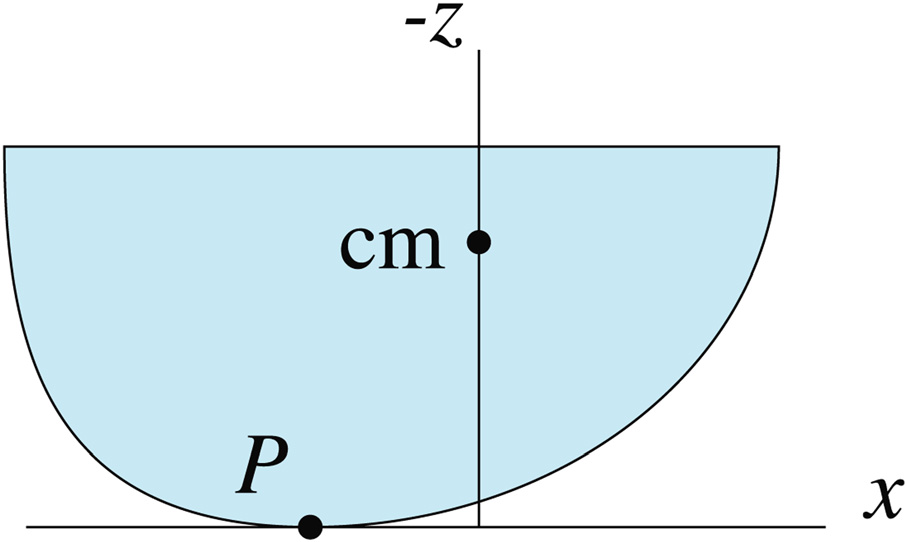
\includegraphics[width=0.7\linewidth]{res/coupe}
		\caption{Vu en coupe du rattleback pendant une oscillation autour de l'axe x}{Crédit : Case \& Jalal}
		\label{fig:coupe}
	\end{figure}
	Le centre de masse et le point de contact n'ont pas la même abscisse $x$. Le poids du centre masse crée un moment au point de contact. Ce moment de force tend à mettre en rotation le rattleback autour de l'axe $y$. (Voir \autoref{fig:coupe})\\
	L'expression de ce couple au point P est donnée par :
	\begin{equation}
	\dfrac{dL_{py}}{dt}=-mgx=\dfrac{mgqy}{p}
	\end{equation}
	Cette expression ce calcul très simplement.\\
	Dans le référentiel du laboratoire, la vitesse du centre de masse au premier ordre :
	\begin{align}
	v_x&=a \omega_y\\
	\intertext{D'où selon les auteurs}
	\label{eq:acc-cm}
	\dfrac{dv_x}{dt}&=a\dfrac{d\omega_y}{dt}=\dfrac{gqy}{\beta p a}
	\end{align}
	\textbf{Remarque : } Premier problème ici, en refaisant les calculs, avec les mêmes hypothèses, je ne trouve pas la même expression.\\
	Je trouve : 
	$$\dfrac{dv_x}{dt}=a\dfrac{d\omega_y}{dt}=\dfrac{gqy}{(\beta-1) p a}$$
	Qui plus est, pour le rattleback utilisé $\beta=1,49$ (selon les auteurs). Je vous invite à consulter la \autoref{subsec:acceleration-cm} pour plus d'explications sur les calculs que j'ai effectués. Dans l'éventualité où mon expression serait correcte, il faudrait en tenir compte et corriger les résultats découlant de cette expression.
	
	L'accélération du centre de masse est équivalente à une force.
	Le couple produit par cette force tend à mettre en rotation le rattleback autour de l'axe z.\\
	
	\textbf{Remarque : }Pour que le couple mette effectivement l'objet en rotation, il faut supposer que le point de contact ne glisse pas. Intervient alors l'hypothèse que les frottements sont suffisants pour empêcher le glissement. Cette hypothèse est admise par les auteurs. La démonstration serait faisable mais compliquerait beaucoup l'étude. D'un point de vue critique, je pense qu'admettre cette hypothèse est raisonnable puisque l'on peut jouer sur les frottements en changeant la composition du support.
	\\
	
%	\textbf{Remarque :} Un point pouvant prêter à confusion dans l'article est qu'il semblerait que les auteurs aient changé d'axe z en cours de route. En effet dans cette section, les résultats énoncés correspondent à des composantes z de vecteur en orientant celui-ci vers le haut.\\

	On peut calculer la composante du couple tendant à mettre en rotation le rattleback autour de l'axe $z$ :
	%todo : PROBLEME DE SIGNE
	$$\tau=\dfrac{mgqy^2}{\beta p a}$$
 	Là encore, il semblerait y avoir un problème. Je peux sans doute me tromper, mais il semblerait que le signe de cette expression soit incorrect. De plus pour arriver à ce résultat, il faut à priori faire une hypothèse qui ici n'a pas été explicitée par les auteurs. Enfin, le calcul dépendant de l'équation \eqref{eq:acc-cm}, si effectivement mon résultat est correct, il faudrait en plus remplacer $\beta$ par $(\beta-1)$. Là encore je vous invite à consulter le détail des calculs \autoref{subsec:acceleration-angulaire}\\
	À partir de cette expression, on peut trouver (\ref{subsec:acceleration-angulaire})
	\begin{equation}
	\label{eq:moyenne-rot}
		\left<\dfrac{dn}{dt}\right>=\dfrac{gqy_0^2}{2\beta p\gamma a^3}
	\end{equation}
	%Pour plus de détails dans les calculs, voir 
	%si CM accéléré <=> a une force qui s'exerce. La dite force est produite par le point de contacte.
	%On peut calculer le couple résultant de cette force : (32)
	
%	Compte tenu des nombreux problèmes, j'ai voulu faire les applications numériques et les comparer aux observations cependant les observations n'ont pas été données quantitativement pour cette partie.

	\section{Applications numérique}
	Les auteurs ont mesuré les dimensions de leur rattleback pour ensuite en calculer les différentes propriétés/paramètres tels que : les moments d'inerties, les paramètres de courbures ($p$ et $s$) etc.\\
	Avec ses valeurs ils ont pu calculer les fréquences propres $\Omega_x$ et $\Omega_y$ et les comparer à la réalité. Les fréquences réelles sont obtenues à partir d'un enregistrement vidéo de leur rattleback.

	\begin{center}
		\begin{tabular}{lll}
		&	Calcul	&Expérimental\\[4pt]
		$\Omega_x$		&	60,9s$^{-1}$	&47s$^{-1}\pm$9,4\\
		$\Omega_x$		&	8,77s$^{-1}$	&6,3s$^{-1}\pm$1,3
		\end{tabular}
	\end{center}
	Ainsi, compte tenu des nombreuses approximations faites, les résultats sont cohérents avec les observations.
	J'ai été un peu déçu que les auteurs n'aient pas donné les résultats expérimentaux de l'expression \eqref{eq:moyenne-rot}. Il est simplement mentionné dans l'article, qu'en faisant l'application numérique pour $y_0=2mm$,
	$$\left<\dfrac{dn}{dt}\right>=0,5rad.s^{-1}$$
	Ce qui serait cohérent avec leur observations.\\
	Au passage, cette expression est une accélération angulaire et devrait donc être en rad.s$^{-2}$.
	\section{Synthèse}
	
	Dans la première partie, les auteurs ont réussi à montrer que la rotation autour de l'axe z était instable et induisait des perturbations (oscillations) autour des axes horizontaux $x$ et $y$. Cette instabilité dépend du produit $n\times q$ autrement dit du sens de rotation $n$ et de la façon dont est réalisée l'asymétrie $q$.
	
	On montre ensuite que par conservation d'énergie, si il y a oscillation, il y a forcément diminution de l'énergie de rotation. On peut donc parler de conversion de type d'énergie.
	
	Pour finir, à partir d'oscillation on montre que le rattleback entre en rotation. La encore le sens dépend de l'asymétrie (du signe de $q$).
	
	Pour résumer avec des symboles logiques, on pourrait reformuler cela de la manière suivante:
	$$\text{rotation ("mauvais sens")}\implies\text{oscillations}\implies\text{rotation ("bon sens")}$$
	
	\section{Conclusion}
	Pour conclure, ce travail d'analyse d'article scientifique m'a permis de me rendre compte d'un certain nombre de choses.\\
	
	Tout d'abord, la façon dont est construite l'étude menée sur le rattleback me semble relativement naturelle. Je pense que cela vient du fait que nous nous familiarisons avec cette démarche scientifique dans nos études, quel que soit le domaine étudié. N'étant pas très à l'aise en mécanique du solide, il m'a fallu admettre certains résultats, mais qui je trouve n'a pas été très gênant dans la compréhension de l'article. Cela m'a fait réaliser qu'avec les bases de physique acquis à la fin de la licence on peut comprendre ce qui est fait, suivre les étapes de calculs sans forcement être capable de les faire soi-même de A à Z.
	
	Ensuite, la partie consacrée à la reprise des calculs (en annexe) m'a beaucoup plu. En commençant ce travail d'analyse, je n'avais pas spécialement pour objectif de refaire les calculs. Mais de résultat en résultat, je me suis pris au jeu et ma curiosité m'a poussée à comprendre d'où venaient les résultats introduits sans réelle démonstration ni explication très précise.
	%Résultats faux, hésiter pas a me contacter.
	%Aucun erratum, peut etre juste.

	\pagebreak
	\appendix
	\appendixpage
	\section{Développement mathématique}
	\label{sec:calculs}
	Dans cette section, on essaie de retrouver une partie des expressions données par les auteurs, en détaillant au possible les méthodes et les hypothèses pour y parvenir.\\
	Par alléger l'écriture, on pose la définition suivante :
	$$\dfrac{\partial}{\partial x}\equiv\partial_x$$ 
	\subsection{Expression de z}
	\label{subsec:z}
	La formule \eqref{eq:z} est liée à la forme d'ellipsoïde. Dans l'article, les auteurs expliquent que cette équation est tirée des travaux d'Hermann Bondi ("The Rigid Body Dynamics of Unidirectional Spin" de 1986). J'ai donc voulu savoir comment l'obtenir, cependant la démonstration n'est pas détaillé dans les travaux de Bondi.
	Voyons si l'on peut obtenir une relation similaire en partant de l'équation d'un ellipsoïde. Considérons tout d'abord un ellipsoïde symétrique. L'équation d'un point $(x,y,z)$ sur la surface est donnée par:
	\begin{align*}
		\dfrac{x^2}{a^2}&+\dfrac{y^2}{b^2}+\dfrac{z^2}{c^2}=1
		\intertext{Attention, $a$ n'est pas le même que celui dans \eqref{eq:z}. On peut ainsi exprimer}
		z^2	&=c^2\left(1-\dfrac{x^2}{a^2}-\dfrac{y^2}{b^2}\right)\\
		z	&=c \left(1-\dfrac{x^2}{a^2}-\dfrac{y^2}{b^2}\right)^{1/2}
		\intertext{Intervient ici l'hypothèse que $\dfrac{x}{a}$ et $\dfrac{y}{b}$ sont petits pour le point de contact (i.e petites oscillations)}
		\intertext{On peut alors faire un developpement limité.}
		z	&= c \left(1-\dfrac{1}{2}\dfrac{x^2}{a^2}-\dfrac{1}{2}\dfrac{y^2}{b^2}\right)\\
\iff	z	&= c \left(1-\dfrac{1}{2}\dfrac{c^2x^2}{a^2c^2}-\dfrac{1}{2}\dfrac{c^2y^2}{b^2c^2}\right)
		\intertext{On peut alors poser}
		p=\dfrac{c^2}{a^2}\qquad s=\dfrac{c^2}{b^2}
		\intertext{On obtient alors :}
		z	&= c \left(1-\dfrac{1}{2}p\dfrac{x^2}{c^2}-\dfrac{1}{2}s\dfrac{y^2}{c^2}\right)
	\end{align*}
	On retrouve l'expression de Bondi dans le cas où $q=0$ c'est a dire d'un ellipsoïde symétrique. Il faudrait alors montrer dans le cas non symétrique l'apparition du terme "couplé".
	$$q\dfrac{xy}{a^2}$$
	
	\subsection{Vecteur normal $\vec{u}$}
	\label{subsec:u}
	Je n'ai pas compris pourquoi, mais on trouve le vecteur normal $\vec{u}$ \eqref{eq:uNormal} en prenant le gradient de \eqref{eq:z}. En effet :
	\begin{align*}
	\vec{\nabla}\cdot z &= \begin{pmatrix}
	\partial_x\\
	\partial_y\\
	\partial_z
	\end{pmatrix}
	\cdot
	a\left( 1-\dfrac {1} {2}p\left( \dfrac {x} {a}\right) ^{2}-q\dfrac {xy} {a^{2}}-\dfrac {1} {2}s\left( \dfrac {y} {a}\right) ^{2}\right)\\
	&=-\left(\dfrac{px+qy}{a},\dfrac{qx+sy}{a},1\right)
	\end{align*}
	\textbf{Remarque : } Il est dit dans l'article que $\vec{u}$ est le vecteur normal unitaire.
	\begin{quotation}
		<<upward-pointing unit normal u at that point is given, to first
		order in x and y, by...>>
	\end{quotation}
	Or, simplement en constatant que $u_z=1$, on en déduit que le vecteur n'est pas normé. Il faudrait prendre:
	\begin{align*}
	\vec{v} &=\dfrac{\vec{u}}{||u||}\\
	&=\dfrac{\vec{u}}{\sqrt{\left(\dfrac{px+qy}{a}\right)^2+\left( \dfrac{qx+sy}{a}\right)^2+1}}
	\end{align*}
	Cette petite "erreur" n'a pas d'importance sur la suite des calculs puisque la suite découle des équations suivantes :
	\begin{align*}
	\dfrac{d\vec{A}}{dt}&=\dot{\vec{A}}+\vec{\omega}\times\vec{A}\\[4pt]
	\dfrac{d\vec{v}}{dt}&=0
	\intertext{il vient alors :}
	\dfrac{d\vec{v}}{dt}&=\dot{\vec{v}}+\vec{\omega}\times\vec{v}\\
	&=\alpha\dot{\vec{u}}+\vec{\omega}\times\alpha\vec{u}\\
	&=\alpha(\dot{\vec{u}}+\vec{\omega}\times\vec{u})\\
	\intertext{D'où}
	\dot{\vec{u}}+\vec{\omega}\times\vec{u}=0 &\iff \dot{\vec{v}}+\vec{\omega}\times\vec{v}=0
	\end{align*}
	
	\subsection{Vecteur rotation $\vec{\omega}$}
	\label{subsec:omega}
	Pour trouver une expression de $\vec{\omega}$ nous avons besoin d'une propriété sur le produit vectoriel.
	\begin{equation}
	\vec{a}\times(\vec{b}\times\vec{c})=\vec{b}(\vec{a}\cdot\vec{c})-\vec{c}(\vec{a}\cdot\vec{b})
	\end{equation}
	Selon les équations \eqref{eq:bour} et \eqref{eq:uConstant} on a:
	\begin{align*}
	\dot{\vec{u}}+\vec{\omega}\times\vec{u}         &= 0\\
	\vec{u}\times(\dot{\vec{u}}+\vec{\omega}\times\vec{u})     &= 0\\
	\vec{u}\times\dot{\vec{u}}+\vec{u}\times(\vec{\omega}\times\vec{u})  &= 0\\
	\vec{u}\times(\vec{\omega}\times\vec{u})        &=-\vec{u}\times\dot{\vec{u}}\\
	\vec{\omega}(\vec{u}\cdot\vec{u})-\vec{u}(\vec{u}\cdot\vec{\omega})  &=\dot{\vec{u}}\times\vec{u}\\
	\intertext{En prenant $||\vec{u}||=1$ et en posant $\vec{u}\cdot\vec{\omega}\equiv n$}
	\vec{\omega}=\dot{\vec{u}}\times\vec{u}+n\vec{u}
	\end{align*}
	
	L'idée de poser $\vec{u}\cdot\vec{\omega}\equiv n$ m'a posé pas mal de problèmes de compréhension. Je me demandais quel en était l'intérêt, jusqu'à ce que je calcule explicitement $\vec{\omega}$.\\
	\bgroup
	\addtolength{\jot}{5pt}
	\begin{align*}
	\vec{\omega} &= \dot{\vec{u}}\times\vec{u}+n\vec{u}\\
	&=\begin{pmatrix}[2]\dfrac{p\dot{x}+q\dot{y}}{a}\\\dfrac{q\dot{x}+s\dot{y}}{a}\\0\end{pmatrix} \times \begin{pmatrix}[2]\dfrac{px+qy}{a}\\\dfrac{qx+sy}{a}\\1\end{pmatrix} -n\begin{pmatrix}[2]\dfrac{px+qy}{a}\\\dfrac{qx+sy}{a}\\1\end{pmatrix}\\
	%
	&=\begin{pmatrix}[2]
	\dfrac{q\dot{x}+s\dot{y}}{a}-n\dfrac{px+qy}{a}\\
	-\dfrac{p\dot{x}+q\dot{y}}{a}-n\dfrac{qx+sy}{a}\\
	\left(\dfrac{p\dot{x}+q\dot{y}}{a}\right)  \left(\dfrac{qx+sy}{a}\right)  - \left(\dfrac{q\dot{x}+s\dot{y}}{a}\right)  \left( \dfrac{px+qy}{a}\right)  - n
	\end{pmatrix}
	\end{align*}
	Il semblerait que les auteurs aient fait une hypothèse simplificatrice, les termes sous forme de fraction sont d'ordre 1. On a donc $\omega_z\approx-n$.\\
	D'où
	\begin{equation}
	\vec{\omega}=\dfrac{1}{a}\begin{pmatrix}[2]
	q\dot{x}+s\dot{y}-n(px+qy)\\
	-p\dot{x}-q\dot{y}-n(qx+sy)\\
	- na
	\end{pmatrix}
	\end{equation}
	\egroup
	Vérifions si on peut considérer les hypothèses comme valides :
	
	
	On rappelle que $x$ et $y$ représentent les coordonnées horizontales et verticales du point de contact par rapport au centre de masse. On se convint assez facilement que cet écart au centre de masse est petit par rapport aux dimensions de l'objet.On prendra en ordre de grandeur le millimètre.
	
	
	Nous n'avons pas d'information particulière sur les $\dot{x}$ et $\dot{y}$. Cependant les auteurs souhaitent résoudre le problème pour de petites vitesses.
	
	\begin{multicols}{2}
		\noindent
		\begin{align*}
		x&\approx y \approx 10^{-3}m&\\
		p&=0,923&\\
		s&=0,034&\\
		q&=0,1&\\
		a&=7,1.10^{-3}m&\\
		\end{align*}
		\columnbreak
		\begin{align*}
		\dfrac{qx+sy}{a}&\approx0,06\\[2em]
		\dfrac{px+qy}{a}&\approx0,27
		\end{align*}
	\end{multicols}
	\vspace*{-3em}
	On peut supposer que les termes en $\dot{x}$ et $\dot{y}$ sont également du même ordre.\\
	On peut considérer que $|\omega_z|\approx\pi$ (i.e 1/2 tour par seconde).\\
	L'hypothèse de considérer $\omega_z\approx-n$ semble alors plausible.
	
	%todo calc de v ?
	
	
	\subsection{Moment cinétique et moments de force}
	\label{subsec:moments}
	On cherche à obtenir une relation entre moments de forces (exprimés au barycentre) et moment cinétique. Les quantités sont exprimées dans le référentiel du laboratoire supposé galiléen.
	On part de:
	\begin{align*}
	\vec{L}     &= \vec{r}\times \vec{p}\\
	\iff\dfrac{d\vec{L}}{dt} &= \dfrac{d}{dt}(\vec{r}\times \vec{p})\\
	\iff\dfrac{d\vec{L}}{dt} &= \dot{\vec{r}}\times \vec{p}+\vec{r}\times \dfrac{d\vec{p}}{dt}\\
	\intertext{Or $\vec{p}$ et $\dot{\vec{r}}$ sont colinéaires $\implies \dot{\vec{r}}\times \vec{p} = 0$}
	\iff\dfrac{d\vec{L}}{dt} &= \vec{r}\times \dfrac{d\vec{p}}{dt}
	\end{align*}
	De plus $\dfrac{d\vec{p}}{dt}=\Sigma\vec{F}$ (2$^{\mathrm{eme}}$ loi de Newton)
	\begin{equation}
	\iff\dfrac{d\vec{L}}{dt} = \vec{r}\times\Sigma\vec{F}
	\end{equation}
	On retrouve en fait le théorème du moment cinétique.
	
	\subsection{Équations différentielles couplées}
	\label{subsec:dimension-equations}
	Vérifions que les équations \eqref{eq:equa-diff-couplées1} et \eqref{eq:equa-diff-couplées2} sont cohérentes d'un point de vue dimensionnel.\\
	On rappelle que les paramètres $p,s,q$ sont sans dimension.\\
	Il en est de même pour les paramètres $\alpha,\beta,\gamma$.\\
	En effet, ils s'écrivent sous la forme $\dfrac{I}{ma^2}$
	\begin{align*}
	\implies [\alpha]=[\beta]=[\gamma]=\dfrac{M.L^2}{M.L^2}=1
	\end{align*}
	On rappelle également que $n$ est par définition \eqref{subsec:omega} une vitesse angulaire $[n]=T^{-1}$.\\
	Ainsi chaque terme de \eqref{eq:equa-diff-couplées1} et \eqref{eq:equa-diff-couplées2} est homogène à une accélération.
	%\subsection{De l'oscillation à la rotation}
	
	\subsection{Pulsations propres}
	\label{subsec:pulsations-propres}
	Dans le cas où l'on considère l'objet au repos ($n=0$) et parfaitement symétrique ($q=0$), les équations \eqref{eq:equa-diff-couplées1} et \eqref{eq:equa-diff-couplées2} deviennent :
	
	\[
	\begin{cases}
	s\ddot{y}\alpha=\dfrac{g}{a}(-y(1-s))\\[2ex]
	-p\ddot{x}\beta=\dfrac{g}{a}(x(1-p))
	\end{cases}
	\iff
	\begin{cases}
	\ddot{y}+\dfrac{g}{as\alpha}(1-s)y=0\\[2ex]
	\ddot{x}+\dfrac{g}{ap\beta}(1-p)x=0
	\end{cases}
	\]
	On rappelle que par construction/définition : $0<p<1$ et $0<s<1$ et de même $g,a,\alpha$ sont strictement positifs.\\
	
	On peut donc poser
	\begin{align*}
	\Omega_x^2&=\dfrac{g(1-s)}{as\alpha}\\[2ex]
	\Omega_y^2&=\dfrac{g(1-p)}{ap\beta}
	\end{align*}
	On reconnait alors les équations bien connues (oscillateurs harmoniques)
	\[
	\begin{cases}
	\ddot{y}+\Omega_x^2\ y=0\\[2ex]
	\ddot{x}+\Omega_y^2\ x=0
	\end{cases}
	\]
	Le fait que les indices soient inversés est normal, en effet, c'est la rotation autour de l'axe $x$ qui induit une variation de $y$. Même raisonnement pour $x$.\\
	Et donc $\Omega_x$ et $\Omega_y$ sont les pulsations propres de l'objet.
	
	\subsection{Accélération du centre de masse}
	\label{subsec:acceleration-cm}
	En partant des hypothèses suivantes (résultats donnés par les auteurs) :
	$$\dfrac{dL_{py}}{dt}=\dfrac{mgqy}{p} \qquad \beta=\dfrac{I_y}{ma^2}+1$$
	Et en appliquant le principe fondamental de la dynamique, on a la relation suivante:
	\begin{align}
				\dfrac{dL_{py}}{dt}			&=I_y\dfrac{d\omega_y}{dt}\nonumber\\
		\iff	\dfrac{mgqy}{p}				&=(\beta-1)ma^2\dfrac{d\omega_y}{dt}\nonumber\\
		\label{eq:erreur}
		\iff	\dfrac{mgqy}{pa(\beta-1)}	&=a\dfrac{d\omega_y}{dt}
	\end{align}
	Or les auteurs ont introduit
	$$\dfrac{mgqy}{pa\beta}	=a\dfrac{d\omega_y}{dt}$$
	Je me suis demandé si on avait $\beta \gg 1$. Pour le rattleback considéré, les auteurs ont calculé et trouvé : $\beta = 1,49$. Cet écart entre les deux formules est non négligeable. En supposant tous les autres paramètres constants, on peut comparer :
	\begin{align*}
		f(x)=\dfrac{x}{\beta}&\qquad g(x)=\dfrac{x}{\beta-1}\\
	\iff\dfrac{g}{f}&=\dfrac{\beta}{\beta-1}
	\intertext{En prenant $\beta=1,49$}\\
	\dfrac{g}{f}&\approx3
	\end{align*}
	%todo Analyse des conséquences de l'erreur
	\subsection{Couple et accélération angulaire}
	\label{subsec:acceleration-angulaire}
%	Selon le principe fondamental de la dynamique on a (ici écrit directement en composante):
%	\begin{align*}
%		\tau_z=I_z\dfrac{d\omega_z}{dt}
%	\end{align*}
%	Où $\tau_z$ est la résultante des couples, $\omega_z$ la vitesse angulaire autour de l'axe $z$ et $I_z$ le moment d'inertie correspondant.
%	
%	Dans notre cas le couple est $\tau$ et est orienté vers les $z$ positifs (i.e vers le bas).\\
%	On a aussi $I_z = ma^2\gamma$ (définition \autopageref{eq:equa-diff-couplées2})\\
%	On trouve donc : 
%	\begin{equation*}
%	\dfrac{\omega_z}{dt}
%	\end{equation*}
	Pour trouver l'expression de $\tau$, il suffit de calculer le moment créer par l'accélération du centre de masse au point de contact. On a alors (au premier ordre) : 
	\begin{align*}
		\vec{T}	&=\vec{r}\times m\dfrac{d\vec{v}}{dt}\\
		\intertext{Or $\tau=T_z$}
		\tau&=m(r_x\dot{v_y}-r_y\dot{v_x})\\
			&=m(x\dot{v_y}-y\dfrac{gqy}{\beta p a})
	\end{align*}
	Pour retrouver le $\tau$ donné par les auteurs $\left(\dfrac{mgqy^2}{\beta p a}\right)$, il faut faire l'hypothèse que $\dot{v_y}=0$. Avec cette hypothèse, on obtient : 
	$$\tau=-\dfrac{mgqy^2}{\beta p a}$$
	On remarque un problème de signe. Ce problème n'est pas dramatique si l'on sait de quoi l'on parle. Il pourrait être dû à un changement d'orientation de l'axe $z$ en cours de route.
	En effet, en conservant l'axe $z$ vers le bas (défini au début de l'analyse), il faut bien un signe moins pour correspondre à ce qui est décrit par les auteurs.
	Autre remarque, si effectivement le résultat \eqref{eq:erreur} est correct il faudrait changer $\beta$ par $(\beta-1)$.
	
	Ensuite, on utilise le principe fondamental de la dynamique pour trouver l'accélération angulaire engendrée par ce couple.
	\begin{align*}
			\tau 					&=I_z\dfrac{d\omega_z}{dt}\\
	\iff	\dfrac{d\omega_z}{dt}	&=\dfrac{\tau}{I_z}
	\intertext{Or $\gamma\equiv\dfrac{I_z}{ma^2}$}
	\iff	\dfrac{d\omega_z}{dt}	&=-\dfrac{mgqy^2}{\beta p a}\dfrac{1}{ma^2I_z}\\
									&=-\dfrac{gqy^2}{\beta p a^3 \gamma}
			\intertext{On a également vu que $n\equiv-\omega_z$. Ainsi,}
			\dfrac{dn}{dt}			&=\dfrac{gqy^2}{\beta p a^3 \gamma}
	\end{align*}
	Les auteurs s'intéressent à la moyenne temporelle de cette expression. De plus ils prennent comme hypothèse que $q$ étant petit, $y$ obéit à l'expression d'un oscillateur harmonique.
	$$y=y_0\cos(wt+\phi)$$
	\begin{align}
		\left<\dfrac{dn}{dt}\right>	&=\left<\dfrac{gqy^2}{\beta p a^3 \gamma}\right>\nonumber\\
									&=\dfrac{gqy_0^2}{\beta p a^3 \gamma} \left<\cos^2(wt+\phi)\right>\nonumber\\
		\intertext{En prenant la moyenne temporelle sur une période}
		\left<\cos^2(wt+\phi)\right>&=\dfrac{1}{2}\nonumber\\
		\implies \left<\dfrac{dn}{dt}\right>	&=\dfrac{gqy_0^2}{2\beta p a^3 \gamma}
	\end{align}
\end{document}
% Ils disent qu'ils n'ont pas forcément été plus loin dans l'analyse que leur prédeccesseur mais qu'a l'aide de bonnes approximations, ils ont pu grandement alleger les calculs et ainsi arrivé plus rapidement et facilement a un resultat.
%beaucoup d'autres articles qui traite le probleme en partant des memes bases mais par exemple préférence matricielle
%todo : ouverture sur autres objets étranges. Gömböc, disque d'euler, gyroscope